% fig_locality.tex
% Scatter plot of traversal locality vs test bpd.
% Data from traversal_study.ipynb (Runs 1+2) and novel_arch_study.ipynb (Run 3).
% All points at N=1024, 30 epochs, path-only PE.

\begin{figure}[t]
\centering
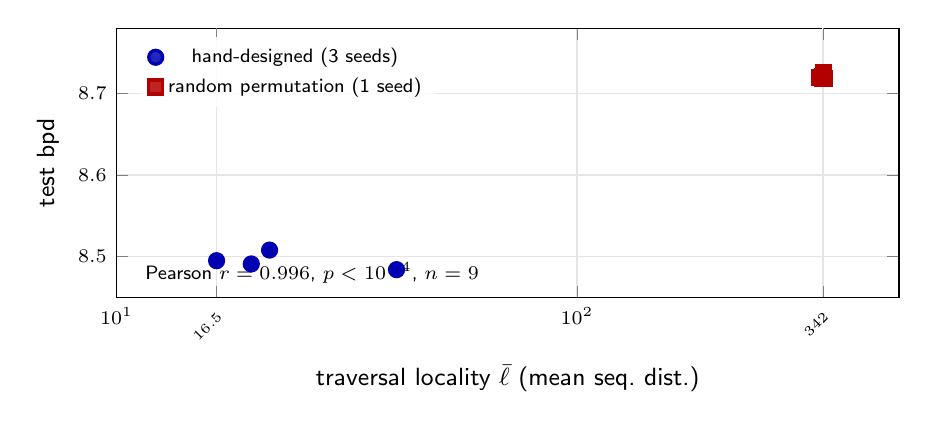
\begin{tikzpicture}
\begin{axis}[
    width=0.95\columnwidth,
    height=5cm,
    xlabel={traversal locality $\bar{\ell}$ (mean seq.\ dist.)},
    ylabel={test bpd},
    xmode=log,
    log basis x=10,
    xmin=10, xmax=500,
    ymin=8.45, ymax=8.78,
    xtick={10,100},
    extra x ticks={16.5,342},
    extra x tick labels={$16.5$,$342$},
    extra x tick style={tick label style={font=\sffamily\tiny,
                        rotate=45, anchor=north east}},
    grid=major,
    grid style={gray!20},
    legend pos=north west,
    legend style={font=\sffamily\scriptsize, draw=none,
                  fill=white, fill opacity=0.85, text opacity=1},
    label style={font=\sffamily\small},
    tick label style={font=\sffamily\scriptsize},
    every axis plot/.append style={very thick},
]

% hand-designed traversals (3 seeds each, mean bpd)
\addplot[only marks, mark=*, mark size=2.5pt, color=blue!70!black]
  coordinates {
    (16.5,  8.495)
    (19.625, 8.491)
    (21.5,  8.508)
    (40.5625, 8.484)
  };
\addlegendentry{hand-designed (3 seeds)}

% random pixel permutations (1 seed each)
\addplot[only marks, mark=square*, mark size=2.5pt, color=red!70!black]
  coordinates {
    (342.1, 8.7202)
    (341.3, 8.7189)
    (345.0, 8.7186)
    (342.3, 8.7254)
    (337.0, 8.7193)
  };
\addlegendentry{random permutation (1 seed)}

% Pearson r annotation
\node[font=\sffamily\scriptsize, anchor=south west]
  at (axis cs:11, 8.455)
  {Pearson $r=0.996$,\ $p<10^{-4}$,\ $n=9$};

\end{axis}
\end{tikzpicture}
\caption{Traversal locality $\bar{\ell}$ (mean sequence distance
  between four-neighbour pixel pairs) vs.\ test bpd on Oxford
  Flowers $32{\times}32$, $N{=}1024$, 30 epochs.
  Hand-designed paths (blue circles) cluster at
  $\bar{\ell}\in[16.5,\,40.6]$ and bpd $\in[8.48,\,8.51]$,
  which is statistically indistinguishable.
  Random pixel permutations (red squares) cluster at
  $\bar{\ell}\approx 342$ and bpd $\approx 8.72$.
  Across the full $20{\times}$ range the relationship is nearly
  linear in $\log\bar{\ell}$ (Pearson $r{=}0.996$,
  $p<10^{-4}$, $n{=}9$), identifying 1D-serialisation of 2D
  structure as the dominant bottleneck.}
\label{fig:locality}
\end{figure}
